\scanpage{23}

\begin{flushright}
\texttt{AVANCE SUR PROGRAMMATION AU 26/0}
\end{flushright}

\texttt{MAIN-D'OEUVRE NECESSAIRES A LA FABRICATION DE 1 S}

\begin{tabular}{lll}
002&TRONCONNAGE ALU&0,18 HEURES\\
004&POINCONNAGE ALU&0,18 HEURES\\
013&SOUDURE SKYDOME&0,34 HEURES\\
020&EBARBAGE&0,20 HEURES\\
021&PLAQUES&0,16 HEURES\\
025&COLLAGE&0,42 \unsure{HEURES}\\
026&MONTAGE SKYDOME&1,0\unsure{8} \unsure{HEURES}
\end{tabular}

\texttt{CHARGE GLOBALE MAIN-D OEUVRE POUR \unsure{LA FABRICATION} DE}

\texttt{COUT PRODUCTION \quad \unsure{418,60|418.60} FRS \quad \unsure{PRIX DE CES}}

\figure{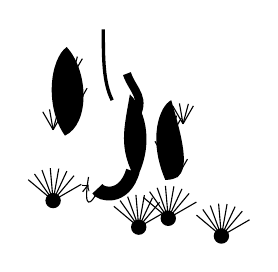
\begin{tikzpicture}[scale=.75]
\fill (0,1.1)..controls(-.35,1.6)and(-.25,2.4)..(.03,2.6)..controls(.4,2.2)and(.43,1.3)..(0,1.1);
\fill (1.2,.35)..controls(.9,.9)and(1,1.2)..(1.1,1.8)..controls(1.4,1.5)and(1.5,.9)..(1.2,.35);
\draw[very thick] (.8,1.7)..controls(.65,2)and(.65,2.4)..(.65,2.9);
\draw[line width=3pt] (1.16,1.35)..controls(1.4,1.75)and(1.15,1.85)..(1.05,2.15);
\draw[line width=5pt] (1.15,.5)..controls(1,0)and(.6,.1)..(.55,.2);
\fill (1.7,.35)..controls(1.4,1.05)and(1.6,1.6)..(1.8,1.7)..controls(2.1,.7)and(2.1,.35)..(1.7,.35);
\foreach \x/\y in {-.2/1.2,0/1.7,.12/2.1,.2/1.6,1.7/.7,1.8/1.1,1.9/.4,2/1.3}{
\foreach \a in {60,75,100,120}{\draw[thin] (\x,\y)--++(\a:.35);}}
\foreach \x/\y in {-.2/0,1.25/-.45,1.75/-.3,2.65/-.6}{
\fill (\x,\y) ellipse (.13 and .13);
\foreach \a in {30,50,65,80,95,110,125,140}{\draw (\x,\y)--++(\a:.55);}}
\draw (.4,.4)..controls(.3,-.2)and(.45,-.05)..(.55,.15);
\draw[->] (.3,.15)--(.4,.27);
\end{tikzpicture}}

\figure{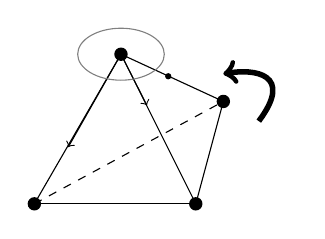
\begin{tikzpicture}[scale=1]
\coordinate (A) at (0,0); \coordinate (B) at (1.1,1.9);
\coordinate (C) at (2.05,0); \coordinate (D) at (2.4,1.3);
\draw (A)--(B)--(C)--(D)--(B);
\draw[thin] (A)--(C);
\draw[dashed] (A)--(D);
\foreach \p in {A,B,C,D}{\fill (\p) circle (.085);}
\draw[->] (B)--(.43,.72);
\draw[->] (B)--(1.43,1.25);
\fill (1.7,1.62) circle (.04);
\draw[gray] (B) ellipse (.55 and .33);
\draw[line width=2pt,->] (2.85,1.05)..controls(3.3,1.65)and(2.8,1.72)..(2.4,1.65);
\end{tikzpicture}}

\diagram{\begin{tikzcd}[column sep=small]
\left.\begin{array}{l}\deleted{\unsure{4|6}\text{ hexagones}}\\\deleted{4\text{ sommets}}\end{array}\right\}
\arrow[r,bend left]
&
\begin{array}{l}
8\text{ triangles}\\
4\text{ sommets d'ordre }6\\
12\text{ arêtes}
\end{array}
\end{tikzcd}}

\[
\unsure{A_4|\mathfrak S_4}
\]

\[
\deleted{\unsure{\widetilde{\mathfrak S}_3}}:
\qquad \unsure{\mu_6|\mathbb H_6}\times(\mathbb Z/2\mathbb Z)^2
\]
\[
\unsure{\mu_4|\mathbb H_4}\times(\mathbb Z/2\mathbb Z)^2
\]

\uline{Hexagone}

\uline{orienté}

\figure{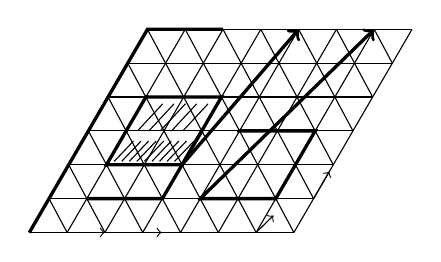
\begin{tikzpicture}[x={(.48cm,0cm)},y={(.25cm,.43cm)}]
\foreach \y in {0,...,6}{\draw (0,\y)--(7,\y);}
\foreach \x in {0,...,7}{\draw (\x,0)--(\x,6);}
\foreach \s in {1,...,12}{
\draw ({max(0,\s-6)},{min(6,\s)})--({min(7,\s)},{max(0,\s-7)});
}
\draw[very thick] (0,0)--(0,6)--(2,6);
\draw[very thick] (1,2)--(1,4)--(3,4)--(3,2)--cycle;
\draw[very thick,->] (3,2)--(4,6);
\draw[very thick,->] (4,1)--(6,6);
\draw[very thick] (4,1)--(6,1)--(6,3)--(4,3);
\draw[very thick] (1,1)--(3,1)--(3,3);
\foreach \x in {1.15,1.35,1.55,1.75,1.95,2.15,2.35,2.55,2.75}{\draw[thin] (\x,2.1)--(\x+.2,2.7);}
\foreach \x in {1.3,1.6,1.9,2.2,2.5}{\draw[thin] (\x,3)--(\x+.25,3.8);}
\draw[->] (1,0)--(2,0); \draw[->] (3,0)--(3.5,0);
\draw[->] (6,0)--(6.2,.5); \draw[->] (7,1)--(7,1.8);
\foreach \p in {(1,2),(1,4),(3,4),(3,2),(4,1),(6,1),(6,3),(4,3)}{\fill \p circle (.06);}
\end{tikzpicture}}

\margin{trois arêtes\\trois sommets}

\uline{Carré orienté}

\figure{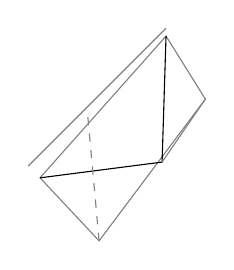
\begin{tikzpicture}[scale=1]
\draw[gray] (0,0)--(1.6,1.8)--(2.1,1)--(.75,-.8)--cycle;
\draw (0,0)--(1.55,.2)--(1.6,1.8);
\draw[gray] (1.55,.2)--(2.1,1);
\draw[dashed,gray] (.75,-.8)--(.6,.85);
\draw[gray] (-.15,.15)--(1.6,1.9);
\end{tikzpicture}}

\figure{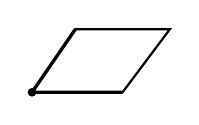
\begin{tikzpicture}[scale=1]
\draw[thick] (0,0)--(.55,.8)--(1.75,.8)--(1.15,0)--cycle;
\draw[very thick] (0,0)--(.55,.8) (0,0)--(1.15,0);
\fill (0,0) circle (.055);
\end{tikzpicture}}

\figure{\begin{tikzpicture}[scale=.8]
\draw[->] (0,1.3)--(0,0);
\draw[gray] (0,1.3)--(1.2,1.3)--(1.2,0);
\draw[gray] (0,1.3)--(.25,1.02);
\end{tikzpicture}}

\figure{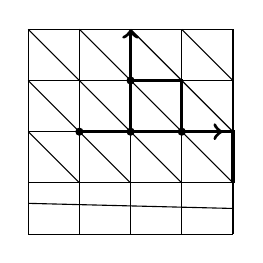
\begin{tikzpicture}[scale=.65]
\foreach \x in {0,1,2,3,4}{\draw (\x,0)--(\x,4);}
\foreach \y in {0,1,2,3,4}{\draw (0,\y)--(4,\y);}
\foreach \x in {0,1,2,3}{\foreach \y in {1,2,3}{\draw (\x,\y+1)--(\x+1,\y);}}
\draw[very thick,->] (2,2)--(2,4);
\draw[very thick,->] (1,2)--(3.8,2);
\draw[very thick] (2,3)--(3,3)--(3,2)--(4,2)--(4,1);
\foreach \p in {(1,2),(2,2),(2,3),(3,2)}{\fill \p circle (.08);}
\draw (0,.6)--(4,.5);
\end{tikzpicture}}

\figure{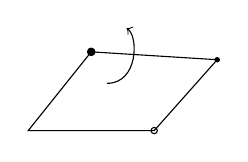
\begin{tikzpicture}[scale=1]
\draw (0,0)--(.8,1)--(2.4,.9)--(1.6,0)--cycle;
\fill (.8,1) circle (.055); \fill (2.4,.9) circle (.035);
\draw (1.6,0) circle (.04);
\draw[->] (1,.6)..controls(1.4,.6)and(1.4,1.2)..(1.25,1.3);
\end{tikzpicture}}

$4$ carrés

$8$ arêtes

$4$ sommets

\fbox{\diagram{\begin{tikzcd}
E_{\varepsilon+}\arrow[r,bend left,very thick]\arrow[d,leftrightarrow,very thick]&
E_{\varepsilon,-}\arrow[l,bend left,very thick]\arrow[d,leftrightarrow,very thick]\\
\overline E_Q\arrow[r,very thick]&\overline E_H
\end{tikzcd}}}

\margin{22}
